\begin{figure*}[t]
  \centering
  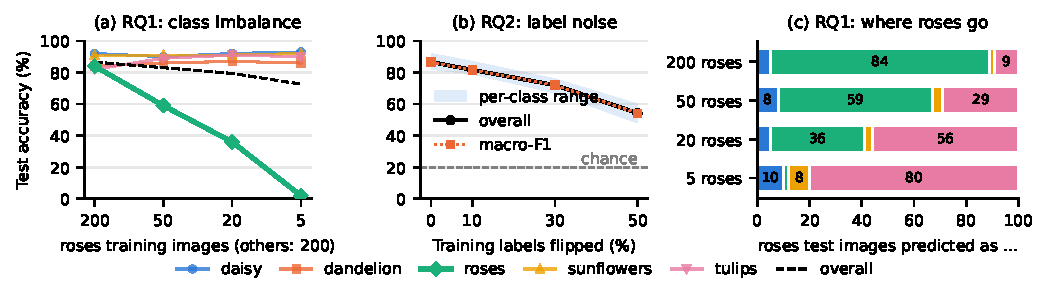
\includegraphics[width=\linewidth]{figures/fig_paper.pdf}
  \vspace{-1.8em}
  \caption{\textbf{(a)} RQ1: per-class test accuracy as roses training images decrease; only roses collapses.
  \textbf{(b)} RQ2: accuracy and macro-F1 (almost identical) as more training labels are flipped.
  The shaded band spans the five per-class accuracies.
  \textbf{(c)} How each RQ1 model classifies the 100 roses test images. The missing roses go mostly to tulips.}
  \label{fig:main}
  \vspace{-0.8em}
\end{figure*}

\section{Introduction}
\label{sec:intro}

A classifier can only learn what its training data shows it.
In practice, that data is often small, dominated by a few common classes, and sprinkled with labeling
mistakes~\cite{buda2018imbalance,song2022noisy}.
Teachable Machine (TM)~\cite{carney2020tm} lets anyone train an image classifier from a few hundred images,
so it is worth knowing how it copes when those images are not ideal.
We study two data-related research questions:

\noindent\textbf{RQ1 (class imbalance).} When one class has far fewer training images than the others,
what happens to its accuracy, and to the accuracy of the other classes?

\noindent\textbf{RQ2 (label noise).} When part of the training labels is wrong, how much does accuracy drop,
and is the drop shared evenly across classes?
